\documentclass{article}

% ==================================================
% FONT -- TIMES STYLE, WORKS WITH PDFLATEX
% ==================================================

\usepackage{newtxtext}
\usepackage{newtxmath}

% ==================================================
% TIKZ
% ==================================================

\usepackage{tikz}

% ==================================================
% COLORS
% ==================================================

\definecolor{navy}{RGB}{20,55,100}

\definecolor{green}{RGB}{45,140,85}
\definecolor{greenpale}{RGB}{230,248,238}

\definecolor{red}{RGB}{190,65,65}
\definecolor{redpale}{RGB}{255,235,235}

% ==================================================
% DOCUMENT
% ==================================================

\begin{document}
	
	\begin{figure}[ht]
		\centering
		
		% ==================================================
		% FIGURE HEADING -- 14 PT
		% ==================================================
		
		{\bfseries\fontsize{14}{17}\selectfont Strengths and Limitations Map}
		
		\vspace{0.45cm}
		
		% ==================================================
		% FIGURE
		% ==================================================
		
		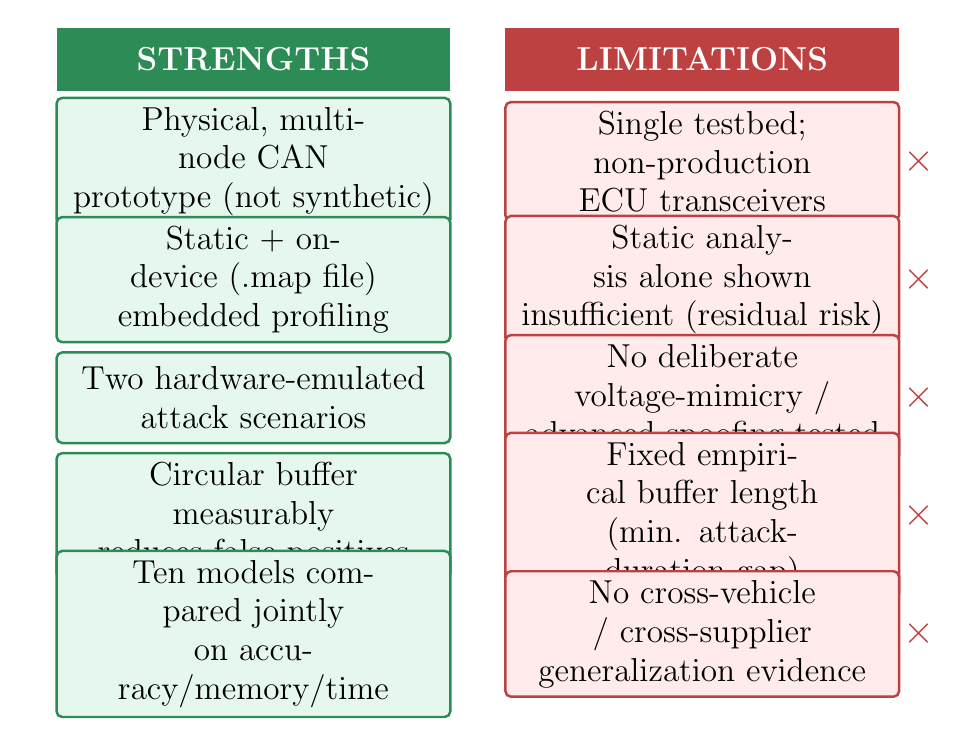
\begin{tikzpicture}[x=1cm,y=1cm]
			
			% ==================================================
			% COLUMN HEADINGS
			% ==================================================
			
			\node[
			rectangle,
			fill=green,
			text=white,
			minimum width=5.0cm,
			minimum height=0.8cm,
			align=center,
			font=\bfseries\fontsize{12}{14}\selectfont
			] (h1) at (0,5.8)
			{STRENGTHS};
			
			\node[
			rectangle,
			fill=red,
			text=white,
			minimum width=5.0cm,
			minimum height=0.8cm,
			align=center,
			font=\bfseries\fontsize{12}{14}\selectfont
			] (h2) at (5.7,5.8)
			{LIMITATIONS};
			
			
			% ==================================================
			% STRENGTH 1
			% ==================================================
			
			\node[
			rectangle,
			rounded corners=2pt,
			draw=green,
			fill=greenpale,
			line width=0.9pt,
			minimum width=5.0cm,
			minimum height=1.15cm,
			text width=4.6cm,
			align=center,
			font=\fontsize{12}{14}\selectfont
			] at (0,4.5)
			{Physical, multi-node CAN\\
				prototype (not synthetic)};
			
			
			% ==================================================
			% LIMITATION 1
			% ==================================================
			
			\node[
			rectangle,
			rounded corners=2pt,
			draw=red,
			fill=redpale,
			line width=0.9pt,
			minimum width=5.0cm,
			minimum height=1.15cm,
			text width=4.6cm,
			align=center,
			font=\fontsize{12}{14}\selectfont
			] at (5.7,4.5)
			{Single testbed; non-production\\
				ECU transceivers};
			
			
			% ==================================================
			% STRENGTH 2
			% ==================================================
			
			\node[
			rectangle,
			rounded corners=2pt,
			draw=green,
			fill=greenpale,
			line width=0.9pt,
			minimum width=5.0cm,
			minimum height=1.15cm,
			text width=4.6cm,
			align=center,
			font=\fontsize{12}{14}\selectfont
			] at (0,3.0)
			{Static + on-device (.map file)\\
				embedded profiling};
			
			
			% ==================================================
			% LIMITATION 2
			% ==================================================
			
			\node[
			rectangle,
			rounded corners=2pt,
			draw=red,
			fill=redpale,
			line width=0.9pt,
			minimum width=5.0cm,
			minimum height=1.15cm,
			text width=4.6cm,
			align=center,
			font=\fontsize{12}{14}\selectfont
			] at (5.7,3.0)
			{Static analysis alone shown\\
				insufficient (residual risk)};
			
			
			% ==================================================
			% STRENGTH 3
			% ==================================================
			
			\node[
			rectangle,
			rounded corners=2pt,
			draw=green,
			fill=greenpale,
			line width=0.9pt,
			minimum width=5.0cm,
			minimum height=1.15cm,
			text width=4.6cm,
			align=center,
			font=\fontsize{12}{14}\selectfont
			] at (0,1.5)
			{Two hardware-emulated\\
				attack scenarios};
			
			
			% ==================================================
			% LIMITATION 3
			% ==================================================
			
			\node[
			rectangle,
			rounded corners=2pt,
			draw=red,
			fill=redpale,
			line width=0.9pt,
			minimum width=5.0cm,
			minimum height=1.15cm,
			text width=4.6cm,
			align=center,
			font=\fontsize{12}{14}\selectfont
			] at (5.7,1.5)
			{No deliberate voltage-mimicry /\\
				advanced spoofing tested};
			
			
			% ==================================================
			% STRENGTH 4
			% ==================================================
			
			\node[
			rectangle,
			rounded corners=2pt,
			draw=green,
			fill=greenpale,
			line width=0.9pt,
			minimum width=5.0cm,
			minimum height=1.15cm,
			text width=4.6cm,
			align=center,
			font=\fontsize{12}{14}\selectfont
			] at (0,0)
			{Circular buffer measurably\\
				reduces false positives};
			
			
			% ==================================================
			% LIMITATION 4
			% ==================================================
			
			\node[
			rectangle,
			rounded corners=2pt,
			draw=red,
			fill=redpale,
			line width=0.9pt,
			minimum width=5.0cm,
			minimum height=1.15cm,
			text width=4.6cm,
			align=center,
			font=\fontsize{12}{14}\selectfont
			] at (5.7,0)
			{Fixed empirical buffer length\\
				(min. attack-duration gap)};
			
			
			% ==================================================
			% STRENGTH 5
			% ==================================================
			
			\node[
			rectangle,
			rounded corners=2pt,
			draw=green,
			fill=greenpale,
			line width=0.9pt,
			minimum width=5.0cm,
			minimum height=1.15cm,
			text width=4.6cm,
			align=center,
			font=\fontsize{12}{14}\selectfont
			] at (0,-1.5)
			{Ten models compared jointly\\
				on accuracy/memory/time};
			
			
			% ==================================================
			% LIMITATION 5
			% ==================================================
			
			\node[
			rectangle,
			rounded corners=2pt,
			draw=red,
			fill=redpale,
			line width=0.9pt,
			minimum width=5.0cm,
			minimum height=1.15cm,
			text width=4.6cm,
			align=center,
			font=\fontsize{12}{14}\selectfont
			] at (5.7,-1.5)
			{No cross-vehicle / cross-supplier\\
				generalization evidence};
			
			
			% ==================================================
			% CHECK MARKS
			% ==================================================
			
			\foreach \y in {4.5,3.0,1.5,0,-1.5}
			{
				\node[
				font=\bfseries\fontsize{14}{16}\selectfont,
				text=green
				] at (-2.75,\y)
				{$\checkmark$};
			}
			
			
			% ==================================================
			% CROSS MARKS
			% ==================================================
			
			\foreach \y in {4.5,3.0,1.5,0,-1.5}
			{
				\node[
				font=\bfseries\fontsize{14}{16}\selectfont,
				text=red
				] at (8.45,\y)
				{$\times$};
			}
			
		\end{tikzpicture}
		
	\end{figure}
	
\end{document}